\documentclass{article}
\usepackage{graphicx}
\usepackage{amssymb}
\usepackage{amsmath}
\usepackage{tikz}
\usepackage{url}
\usetikzlibrary{shapes}


\linespread{1.4}

\title{Genome Compression Against a Reference \\
        Project Proposal \\}

\author{\\
        Aniruddha Laud (107635282)\\
        Gaurav Menghani (108266803)\\
        Madhava Keralapura (107710538)\\}


\begin{document}

\maketitle

\clearpage
.
\clearpage

\tableofcontents

\clearpage

\section {Introduction}
TODO
\clearpage

\section {Relevant Work}
TODO
\clearpage

\section {Work Done}

\subsection {Storing the Bit Vectors Efficiently}
TODO and add charts

\clearpage

\subsection {Improving the Variable Integer (VINT) storage}
The DNAZip source code makes heavy use of Variable Integer (VINT) storage, so that they do not have to allocate a fixed
number of bits for each integer value that needs to be written. The reason being, if we are writing very small values, and the data type of our choice is the standard integer, we would be using 32 bits for each value that we write but most of the higher bits in the number would not be set. However, if we choose a small data type like a byte, we would not be able to write values greater than $2^8 - 1$. 

This is solved by writing 8 bits at a time, of which the MSB is set if there is another block of 8 bits for the number after the current block. Thus, out of the 8 bits, 1 bit is a flag, and the rest 7 come from the number to be written. We realized that this might not be the most efficient way of doing it. A large number of values written as variable integers are small delta values, and writing 8 bits at a time would mean that atleast 8 bits would be written even if the number is very small. 

The values being written as VINTs during the compression process were written to an auxilliary file. We then tried to compare the space consumed when the size of the VINT word size is varied. 

\begin{figure}[htp]
\centering
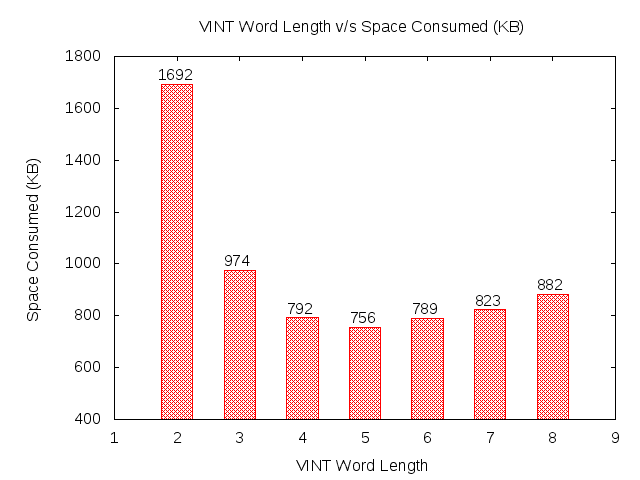
\includegraphics[scale=0.4]{images/VINT.png}
\caption{VINT Word Length v/s Space Consumed (KB)}\label{fig:fs}
\end{figure}

As apparent in the result, using VINT word size of 5 bits was the best choice. The actual compression received from this was 129 KB roughly, which was in line with our expectation before this experiment.

\clearpage

\subsection {Improving the storing of Insertion/Deletion (INDEL)}
After thorough analysis, we realized that the Insertion/Deletion format was pretty packed. One optimization possible was to create a Bit Vector for the Insertions and Deletions which were present in dbSNP.
\clearpage

\section {Conclusion}
TODO
\clearpage

\section {Future Work}
TODO
\clearpage

\begin{thebibliography}{}

\bibitem{jorde04}
  Jorde, Lynn B. and Wooding, Stephen P.,
  \emph{Genetic variation, classification and race}.
  Nature Genetics 36 (11 Suppl): S28–S33. doi:10.1038/ng1435. PMID 15508000,
  2004

\bibitem{ucschg}
  UCSC Genome Bioinformatics, Human (Homo sapiens) Genome Browser Gateway
  http://genome.ucsc.edu/cgi-bin/hgGateway

\bibitem{ucschg18}
  UCSC Genome Bioinformatics, Human Chromosome (hg18)
  http://hgdownload.cse.ucsc.edu/goldenPath/hg18/chromosomes/

\bibitem{dnazip}
  The DNA Zip Project
  http://www.ics.uci.edu/~dnazip/

\bibitem{dnazip_paper}
  Christley, Scott and Lu, Yiming and Li, Chen and Xie, Xiaohui,
  \emph{Human genomes as email attachments}.

\bibitem{gencompress}
  Chen, Xi and Kwong, Sam and Li, Ming,
  \emph{A Compression Algorithm for DNA Sequences and Its Applications in Genome Comparison}
 
\bibitem{jwseq}
  James Watson's Sequence
  http://jimwatsonsequence.cshl.edu/cgi-perl/gbrowse/jwsequence/

\bibitem{completegenomics}
  Complete Genomics
  http://www.completegenomics.com/ 
\end{thebibliography}

\end{document}
